\chapter{Исследовательская часть}

\section{Технические характеристики}

Технические характеристики устройства, на котором выполнялись замеры по времени, представлены далее.

\begin{itemize}
	\item Процессор:2 GHz 4‑ядерный процессор Intel Core i5.
	\item Оперативная память: 16 ГБайт.
	\item Операционная система: macOS Venura 13.5.2. 
\end{itemize}

\section{Прмиер работы}
Демонстрация работы программы приведена на рисунке 4.1

\begin{figure}[h]
	\centering
	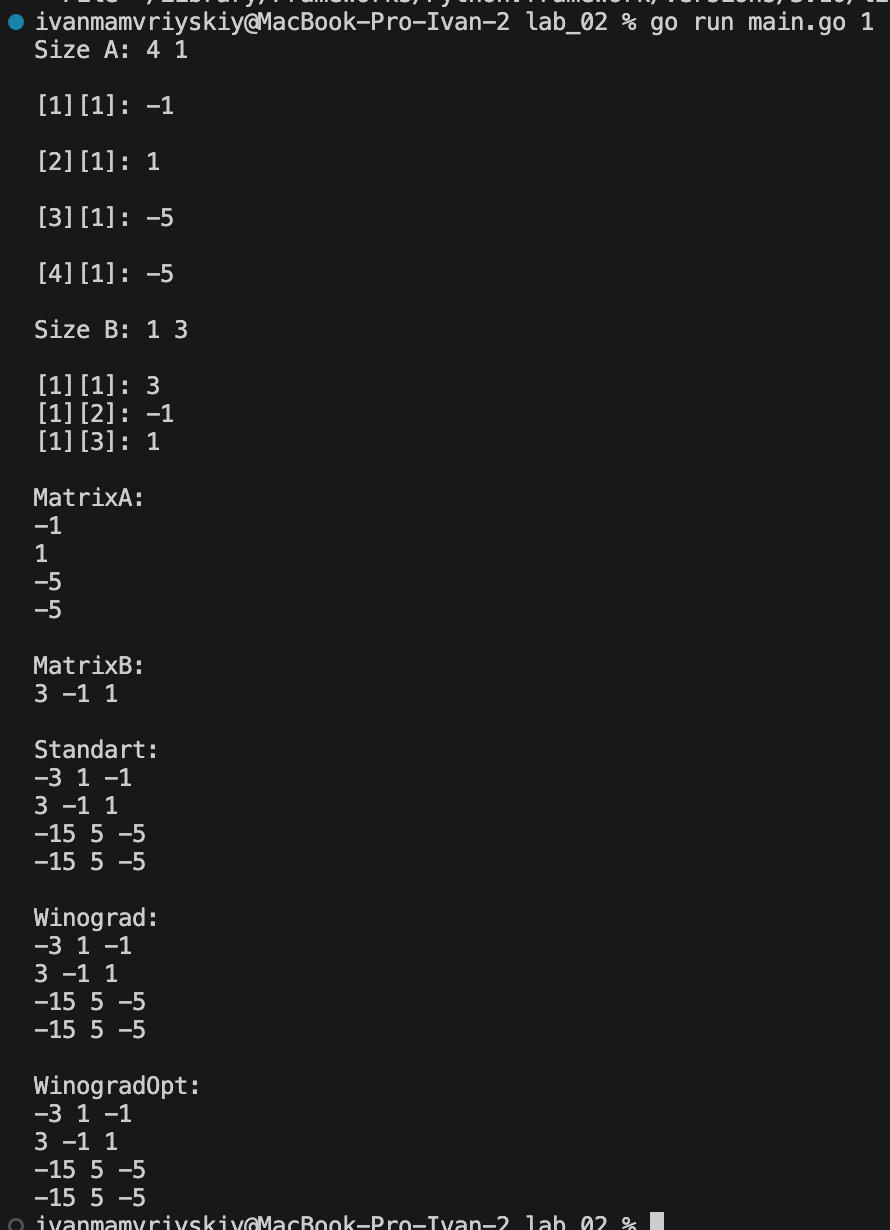
\includegraphics[height=0.4\textheight]{img/example.jpg}
	\caption{Демонстрация работы программы}
	\label{img:demonstration}
\end{figure}

\section{Время выполнения алгоритмов}

\begin{figure}[h]
	\centering
	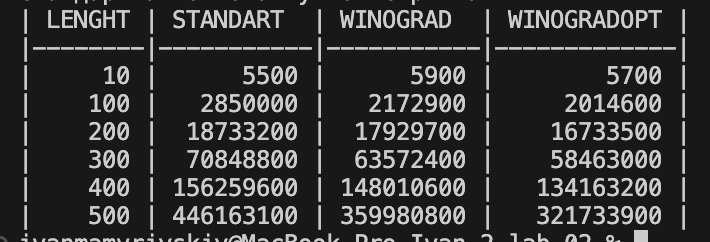
\includegraphics[height=0.15\textheight]{img/resTime.jpg}
	\caption{Результаты замера времени}
	\label{img:demonstration}
\end{figure}

\begin{figure}[h]
	\centering
	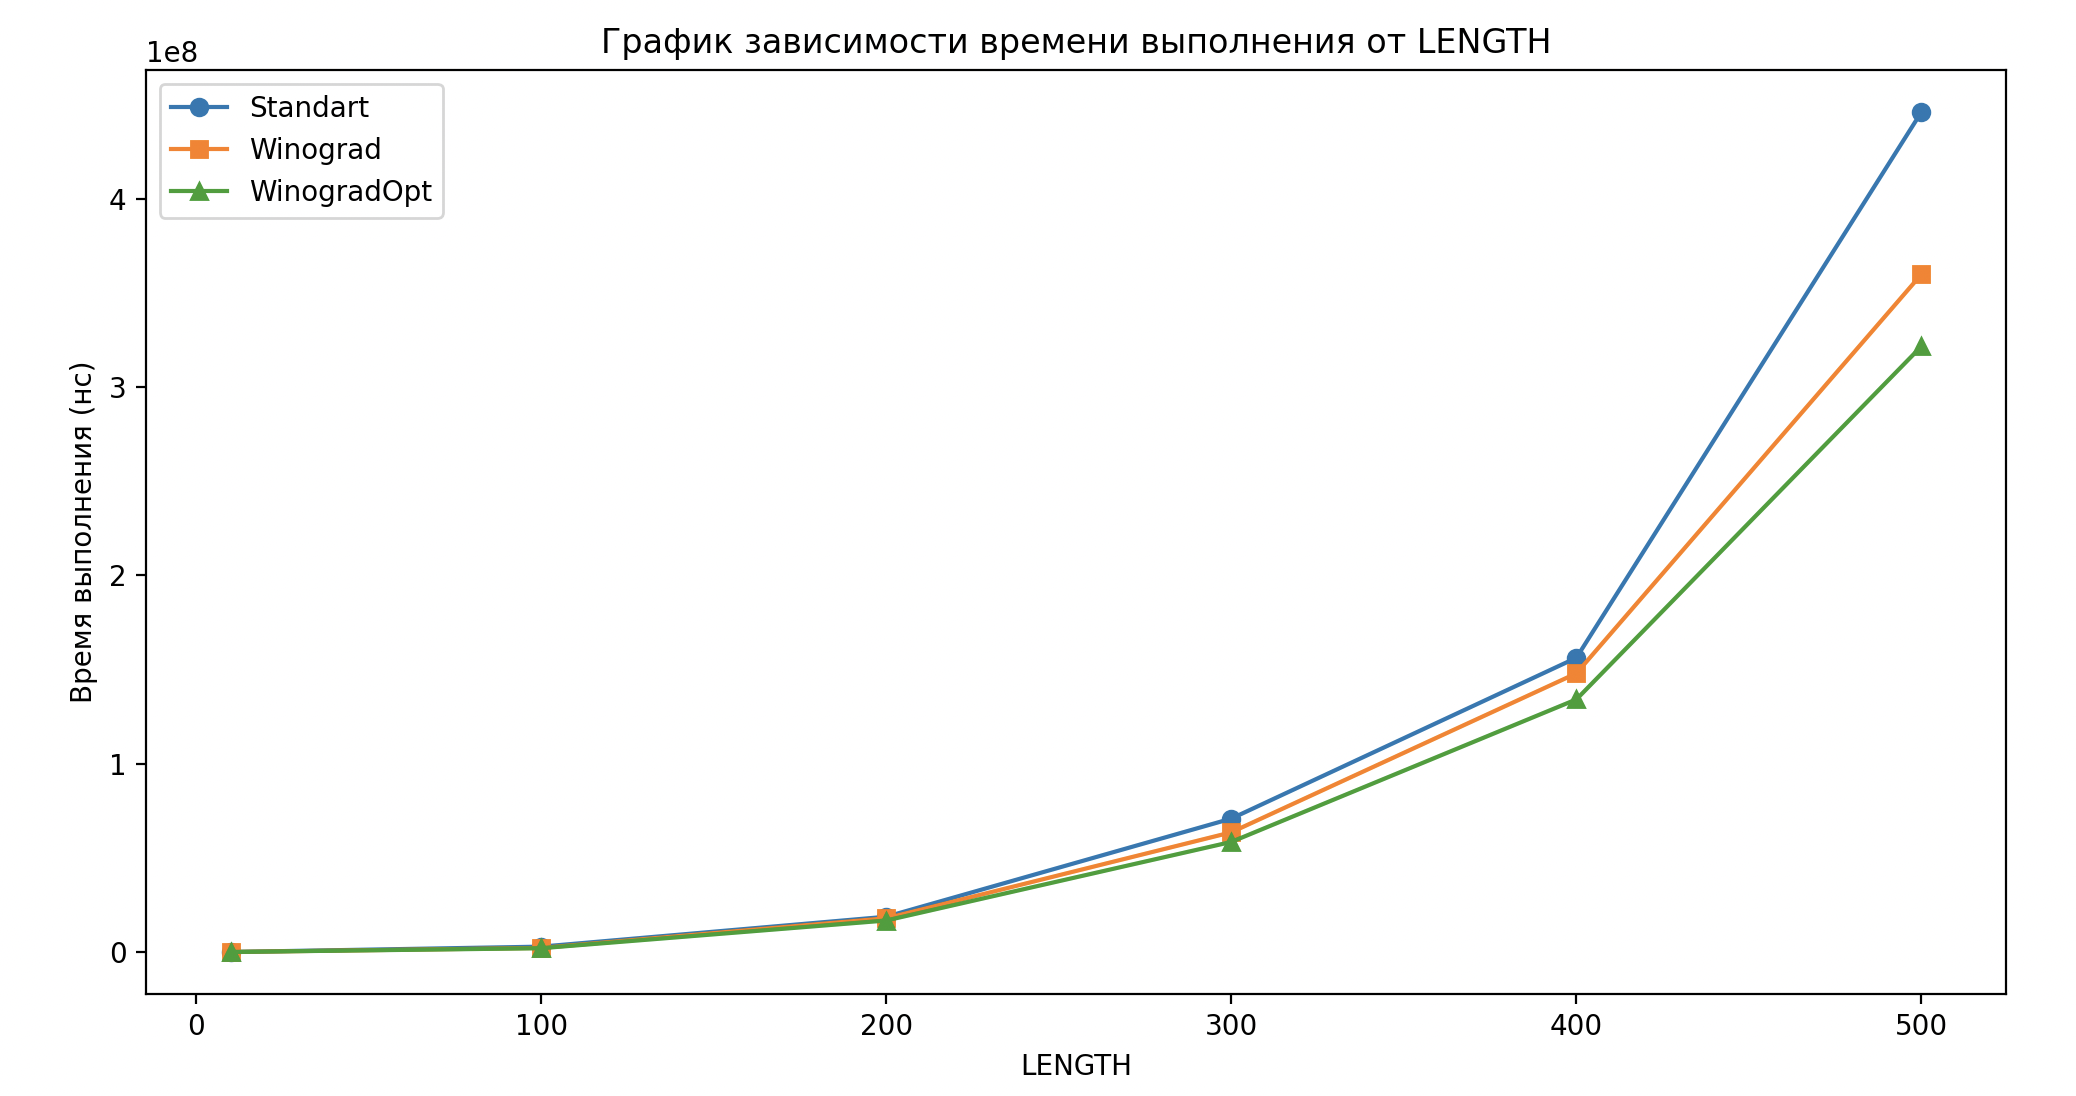
\includegraphics[height=0.37\textheight]{img/graph.jpg}
	\caption{График замера времени}
	\label{img:demonstration}
\end{figure}

\clearpage
\section{Вывод}

По результатам эксперимента можно сделать следующие выводы:
\begin{itemize}[left=\parindent]
     \item прямая реализация алгоритма Винограда без какой-либо опитимизации
         работает примерно в 1.2 раза быстрее стандартного алгоритма;
     \item оптимизированная версия Винограда работает в 1.4 раза быстрее
         стандартного алгоритма.
\end{itemize}

Таким образом, для вычислений произведений матриц при необходимости меньшего времени вычислений 
следует использовать оптимизированный алгоритм Виноградова.


